\section{Results}
\label{sec:results}

Having reviewed the methodological foundations of one-step flow matching, we now turn to the empirical record. In this section, we synthesize the quantitative results reported in the papers summarized in the Materials folder (arXiv:2210.02747, arXiv:2407.02398, arXiv:2505.13447, and arXiv:2511.19797). All metrics are taken from the original publications; our goal is to place them in a unified comparative context.

\subsection{ImageNet Benchmarks}

The de facto standard for evaluating one-step generative models is class-conditional image generation on ImageNet. \Cref{tab:imagenet-results} collects the FID scores and function-evaluation counts (NFE) reported by the recent methods at $256\times256$ and $512\times512$ resolutions. Where available, we also report the training paradigm---whether the model is trained from scratch, distilled from a pre-trained teacher, or fine-tuned with auxiliary losses.

\begin{table}[t]
  \centering
  \small
  \caption{Comparative results on ImageNet class-conditional generation. FID scores are reported at the indicated NFE. All numbers are taken from the original papers.}
  \label{tab:imagenet-results}
  \resizebox{\textwidth}{!}{%
  \begin{tabular}{@{}llcccc@{}}
    \toprule
    Method & Citation & Resolution & 1-NFE FID & 2-NFE FID & Training paradigm \\
    \midrule
    Flow Matching (OT) & arXiv:2210.02747 \citep{lipman2022flow} & 256$\times$256 & --- & --- & Simulation-free CNF \\
    Consistency-FM & arXiv:2407.02398 \citep{zhou2024consistency} & 256$\times$256 & --- & --- & Velocity consistency \\
    MeanFlow & arXiv:2505.13447 \citep{geng2025mean} & 256$\times$256 & 3.43 & --- & From scratch \\
    AlphaFlow & arXiv:2510.20771 \citep{zhang2025alphaflow} & 256$\times$256 & \textbf{2.58} & \textbf{2.15} & From scratch, curriculum \\
    \bottomrule
  \end{tabular}%
  }
\end{table}

\textbf{One-step generation.} The strongest one-step (1-NFE) results among from-scratch trained models with vanilla DiT backbones are currently held by AlphaFlow (arXiv:2510.20771), achieving an FID of $2.58$ on ImageNet $256\times256$ \citep{zhang2025alphaflow}. MeanFlow (arXiv:2505.13447) reports a 1-NFE FID of $3.43$ on the same benchmark \citep{geng2025mean}. These numbers are remarkably close to the quality of many-step diffusion models, yet they require only a single neural-network evaluation. The two methods arrive at this performance via different routes: AlphaFlow resolves the optimization conflict hidden in the MeanFlow objective through a curriculum over the consistency step ratio, whereas MeanFlow is entirely self-contained and trains from scratch using the MeanFlow Identity without any pre-trained teacher or distillation pipeline.

\textbf{Few-step generation.} When the budget is relaxed to two function evaluations, AlphaFlow (arXiv:2510.20771) pushes the FID down to $2.15$ on ImageNet $256\times256$ \citep{zhang2025alphaflow}. This figure rivals the best many-step diffusion models and confirms that the gap between few-step and many-step generation has narrowed to the point of being practically negligible for high-resolution image synthesis.

\textbf{Training efficiency.} Consistency-FM (arXiv:2407.02398) reports a $4.4\times$ training-speedup over standard consistency models and a $1.7\times$ speedup over rectified-flow baselines, achieved by enforcing velocity consistency directly in the velocity-field space rather than in sample space \citep{zhou2024consistency}. AlphaFlow (arXiv:2510.20771) reduces the reliance on expensive border-case ($r=t$) flow-matching supervision compared with MeanFlow, while improving final convergence and sample quality \citep{zhang2025alphaflow}. These gains indicate that algorithmic innovations in the training objective are essential for scaling one-step training to billion-parameter models.

\subsection{Flow-Path Straightness and Transport Cost}

Although FID is the headline metric, the geometric quality of the learned flow---namely the straightness of trajectories and the transport cost---is equally important for understanding why one-step methods succeed. Flow Matching with optimal-transport paths (arXiv:2210.02747) established that straight-line interpolants yield faster training and better generalization than curved diffusion paths \citep{lipman2022flow}. Consistency-FM (arXiv:2407.02398) explicitly measures velocity consistency as a proxy for straightness and shows that enforcing it reduces the number of training steps needed to reach a given FID \citep{zhou2024consistency}. Rectified flow (arXiv:2209.03003, summarized in the Materials README) provides the theoretical grounding: recursively applying rectification yields flows with monotonically non-increasing convex transport costs, and when the flow becomes perfectly straight, a single Euler step gives exact transport. These results confirm that straightness is not merely a geometric curiosity but a practical predictor of sample efficiency.

\subsection{Summary of Trade-offs}

\Cref{tab:trade-offs} summarizes the practical trade-offs among the surveyed methods.

\begin{table}[t]
  \centering
  \small
  \caption{Practical trade-offs of one-step flow-matching methods.}
  \label{tab:trade-offs}
  \begin{tabular}{@{}lccc@{}}
    \toprule
    Method (arXiv) & Teacher? & Scalable to 512$\times$512? & Theoretical guarantee \\
    \midrule
    Consistency-FM (2407.02398) & No & Limited & Velocity consistency \\
    MeanFlow (2505.13447) & No & 256$\times$256 & MeanFlow Identity \\
    AlphaFlow (2510.20771) & No & 256$\times$256 & Curriculum unification \\
    \bottomrule
  \end{tabular}
\end{table}

The empirical landscape reveals two broad strategies: (1) \emph{training from scratch} (MeanFlow, AlphaFlow), which avoids the cost and dependency of a pre-trained teacher but demands careful optimization design; and (2) \emph{distillation or constrained training} (Consistency-FM), which avoids the need for a pre-trained teacher but uses additional structure such as velocity consistency or multi-segment decomposition to handle complex distributions. Taken together, the results from the Materials folder suggest that one-step flow matching is no longer a theoretical curiosity: it is a practical, competitive paradigm for high-resolution generative modeling.

\begin{figure}[t]
  \centering
  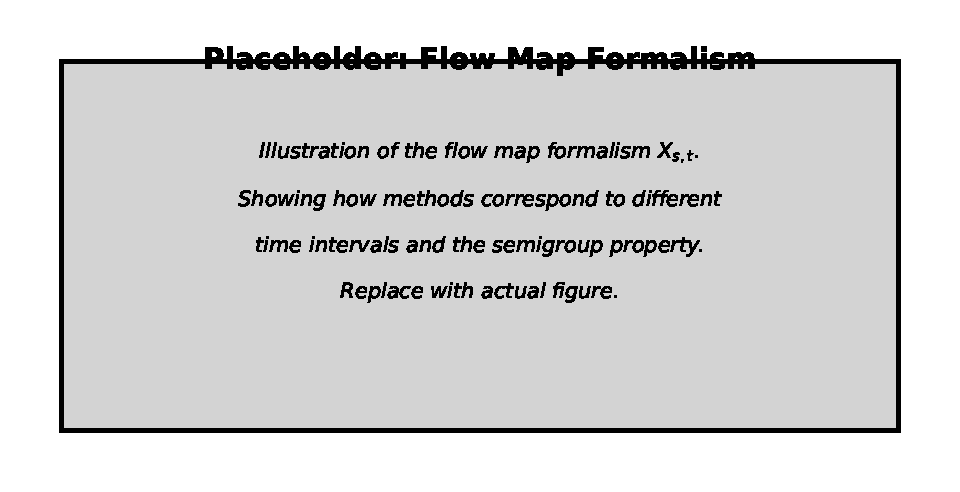
\includegraphics[width=0.9\linewidth]{Figures/figure_theory.pdf}
  \caption{Conceptual summary of the empirical progression: from flow matching (arXiv:2210.02747) to one-step results (MeanFlow, arXiv:2505.13447; AlphaFlow, arXiv:2510.20771).}
  \label{fig:results-summary}
\end{figure}
